\section{The functional reference architecture of the perception chain}\label{sec:refarchitecture}
This section develops a functional reference architecture for the perception chain allowing to provably bound the risk for misperceptions. The following principles guided the development of this architecture:
\begin{enumerate}
\item It must be possible to bound the contributions to risks for each component of the perception chain.
\item This entails the need to specify for each element in the perception the conditions under which this element can be \enquote{trusted}. Violations of such conditions must be monitored and --if persistent-- must induce declaration of \enquote{blindness}, automatically inducing minimal risk maneuvers.
\item The reference architecture must provide guidance as to the degree of precision of perception required for current maneuver decisions.
\item The reference architecture must support trade-off between maximal availability and maximal safety.
\end{enumerate}
We discuss the implications of these design principles in separate subsections, along the flow through the perception chain.
\subsection{Quality criteria for sensor components}\label{subsec:quality}
While radar systems are widely deployed for variants of ACC systems and emergency breaking systems, their integration in level 3, 4, or 5 HAV constitutes a completely different operational context, because the overall safety case can no longer rely on human supervision of the \modify{environment of the ego car}{car's environment}. Well known phenomena such as ghost objects stemming from undesired and uncontrollable reflections, or \enquote{stealth type cars} such as the VW beetle, or simply reflections\del{ induced} by metal-coating of truck planes are but examples of a plethora of phenomena, which all influence quality of object detection through radar. With the transition to HAV, quality criteria must quantify the risks of missing objects, or showing ghost objects. Similar types of distortion of perception are documented a.o. under rain conditions~\cite{Cord14}, for video systems in certain types of lighting conditions, etc. We propose a uniform quality measure for different type of sensor systems, by assessing their capability to detect all relevant objects in what is often called the \emph{occupancy grid} enclosing the ego car. We take a suitable 3d extension of the electronic horizon of the ego vehicle, assume a sufficiently fine grained, not necessarily homogeneous partitioning of this 3d space, and refer to this as \emph{occupancy grid(ego)}. We view sensors as labelling partitions of the occupancy grid, providing information about whether a given sensor has identified some artifact in this grid partition, depending on sensor type filled with additional information such as speed (for radar), temperature (for infrared), gray-scale distribution of pixels for video cameras, \del{\ldots}typically as distributions with confidence levels, e.g. regarding the likelihood of some artifact being located in this grid partition. 

We provide a formal quality requirement on sensors by adapting the safe perception requirement in formula (1). Specifically, for a given position \textit{pos}  of sensor  \textit{s}  on vehicle ego, let us denote by \textit{visible(s,pos)} the coherent subspace of the occupancy grid covered by sensor \textit{s} when mounted at this position. Then for any relevant artifact  $a$, and any property  \textit{label($a$)} discernable by  \textit{s}  in this position, we would want the sensor \textit{s} to almost always, up to some bounded risk $r_s$, correctly label the grid field with \textit{label($a$)} at time $t$, when $a$ is at a visible grid partition in ground truth, as determined by the state of \textit{TS(ego)} at that point in time:
\begin{align}\label{eq:safelabelling(s,pos)}
    &\textit{Safe}\_\textit{labelling(s,pos)} \equiv 					\\		
 & \forall a\in\textit{ observables(TS(ego))}\forall p \in \textit{occupancy grid(ego)}: \Box(\textit{relevant(a)} \land \nonumber\\  
& \land a \textit{ is at } p\land p\in \textit{visible(s,pos)} \Rightarrow P(\neg( \Box_{\leq\Delta} d_{a,s}(a,\textit{label}(a))\leq\delta_{a,s}))) < r_s\nonumber
\end{align}
In this formula, we interpret the predicate \textit{visible(s,pos)} \emph{dynamically}, providing for subspaces of the occupancy grid to be temporarily blocked through artifacts such as other vehicles, or buildings, etc. Moreover, since phenomena such as glare, fog, heavy rain etc will have strong negative impact on achieving sufficiently precise distances between beliefs and ground truth, we propose to characterize for each sensor what we call \emph{adverse} conditions. Only by using advanced sensor-systems (such as radar)  capable of identifying most ghost objects, and explicating adverse conditions, can we obtain a sufficiently tight bound on the risks of incorrect labelling of the occupancy grid, to achieve an overall risk tolerated by society. The down side is the need to then also identify reliably such adverse conditions; in this paper, we integrate such adverse conditions in our ontology, and then use the full power of the perception chain to learn sufficiently reliable classifications of adverse conditions, see next subsection. As in \cite{galbas}, we propose to use learning techniques from field observations to characterize adverse conditions for each sensor \textit{s} and to derive such quality guarantees. We now weaken formula (2) by weakening the criteria for sufficient precision of beliefs in that no promises regarding precision are made when adverse conditions $ad$ occur:
\begin{align}\label{eq:safelabelling(s,pos,ad)}
&\textit{Safe}\_\textit{labelling(s,pos,ad)} \equiv\forall a\in \textit{observables(TS(ego))}\\  	
&\forall p\in\textit{occupancy grid(ego)}   :\Box(\textit{relevant(a)} \land a\textit{ is at p }\land \nonumber\\
& p\in\textit{visible(s,pos)} \Rightarrow P(\neg(\Box_{\leq\Delta} (d_{a,s}(a, \textit{label(a)})\leq \delta_{a,s}))\textit{ unless } ad)) < r_s\nonumber
\end{align}
Note that we can in particular encode the constraints of a given ODD in such adverse conditions, which thus entails that information of a sensor is not trusted if working outside the constraints of the ODD. OEMs typically compensate for inaccuracies in sensors by redundancy and diversity in sensor systems and by \emph{sensor fusion} involving composed sensors.

We can derive a composed sensor s as the \emph{fusion} of two qualified positioned sensors $<$s1,pos1$>$  and $<$s2,pos2$>$ as follows:
%
\begin{itemize}
\item ad(s) is the disjunction of ad(s1) and ad(s2)
\item visible(s) = visible($<$s1,pos1$>$) $\cup$ visible($<$s2,pos2$>$)
\item for each $p\in $\textit{occupancy grid(ego)}:  \\
if p $\in$ visible($<$s1,pos1$>$) $\cap$ visible($<$s2,pos2$>$) then
\begin{itemize}
\item if $\neg$ad(s1)$\land\neg$ ad(s2) then\\
if label(s1)(p) $\land$ label(s2)(p) $\not=$ false 
\begin{itemize}
\item[] then label(s)(p) := label(s1)(p) $\land $label(s2)(p)
\item[] else label(s)(p) := $\bot$
\end{itemize}
\item[] else if ad(s1)$\land\neg$ad(s2) then label(s)(p) := label(s2)
\item[] else if $\neg$ad(s1)$\land$ad(s2) then label(s)(p) := label(s1)
\item[] else if ad(s1) $\land$ ad(s2) then label(s) := $\bot$
\end{itemize}
\item[] else if p$\in$visible($<$s1,pos1$>$) $\setminus$ visible($<$s2,pos2$>$) then\\	
if $\neg$ad(s1)
\begin{itemize}
    \item[] then label(s) := label(s1)
	\item[] else if ad(s1) then label(s) := $\bot$
	\end{itemize}
	else if p $\in$ visible($<$s2,pos2$>$) $\setminus$ visible($<$s1,pos1$>$) then
	\begin{itemize}
	\item[] if $\neg$ad(s2) 
	\begin{itemize}
	    \item[]then label(s) := label(s2)
	\item[] else if ad(s2) then label(s) := $\bot$
    \end{itemize}
    \end{itemize}
\end{itemize}
The labels are part of an ontology with a lattice structure, cf. Section~\ref{sec:proofrule}. The fusion operator on labels is accordingly based on the classical \emph{meet-semilattice} - We illustrate some cases below:
\modify{\begin{itemize}
    \item parts of the occupancy grids are labelled “free” if all sensors for which this part is visible and which are operating in non-adverse conditions agree on this; 
\item however, if one sensor operating in non-adverse conditions senses one object, while other sensors operating in non-adverse conditions detect no object, the fusion operator yields $\bot$.
\item In general any detected inconsistencies are marked $\bot$. 
\item If, say, front radar and front stereo camera, both working in non-adverse conditions,  agree on identifying an object in a field of the occupancy grid, then the  of meet of their sensor values at this field of the occupancy grid contains the detected position and speed of the object as well as a sequence of vertical slices of a series of matrices of gray values of pixels.
\item Also the combined sensor labels fields p with $\bot$ if p is only visible for one sensor, but this sensor cannot be trusted because of prevailing adverse conditions.
\end{itemize}}{
parts of the occupancy grids are labelled “free” if all sensors for which this part is visible and which are operating in non-adverse conditions agree on this; 
however, if one sensor operating in non-adverse conditions senses one object, while other sensors operating in non-adverse conditions detect no object, the fusion operator yields $\bot$.
In general any detected inconsistencies are marked $\bot$. 
If, say, front radar and front stereo camera, both working in non-adverse conditions,  agree on identifying an object in a field of the occupancy grid, then the fusion of their sensor values at this field of the occupancy grid contains the detected position and speed of the object, as well as a sequence of vertical slices of a series of matrices of gray values of pixels.
Also the combined sensor will label a field p with $\bot$ if p is only visible for one sensor, but this sensor cannot be trusted because of prevailing adverse conditions.
}
For observations where both sensors are in non-adverse conditions, and both sensors observe $p$, then the risk of misperception is reduced to $r_{s1} \times r_{s2}$ if the misperceptions are stochastically independent under operating conditions favourable for both sensors. Otherwise the risk for misperception of the fused system for a field visible to both sensors is min($r_{s1}$,$r_{s2}$).

Level 4 and 5 HAV must guarantee by construction what we call \emph{sensor completeness with maximal risk r}: for all runs of $RUNS(TS(ego))$, there exists a \enquote{sufficiently dense} sequence of time instances $(t_j)$, $j\in \mathbb{N}$ s.t. for all $t_j$ and all relevant fields p of the occupancy grid, there must at least be one positioned sensor operating in non-adverse conditions, such that p is visible for this sensor, and the risk of misperception by this sensor is smaller than r, unless there are multiple positioned sensors all operating in non-adverse conditions, which are stochastically independent under such conditions; in this case the products of their risk levels must be smaller than r. The term \enquote{sufficiently dense} depends on the current ODD.

\subsection{The functional reference architecture}
\begin{figure}
    \centering
    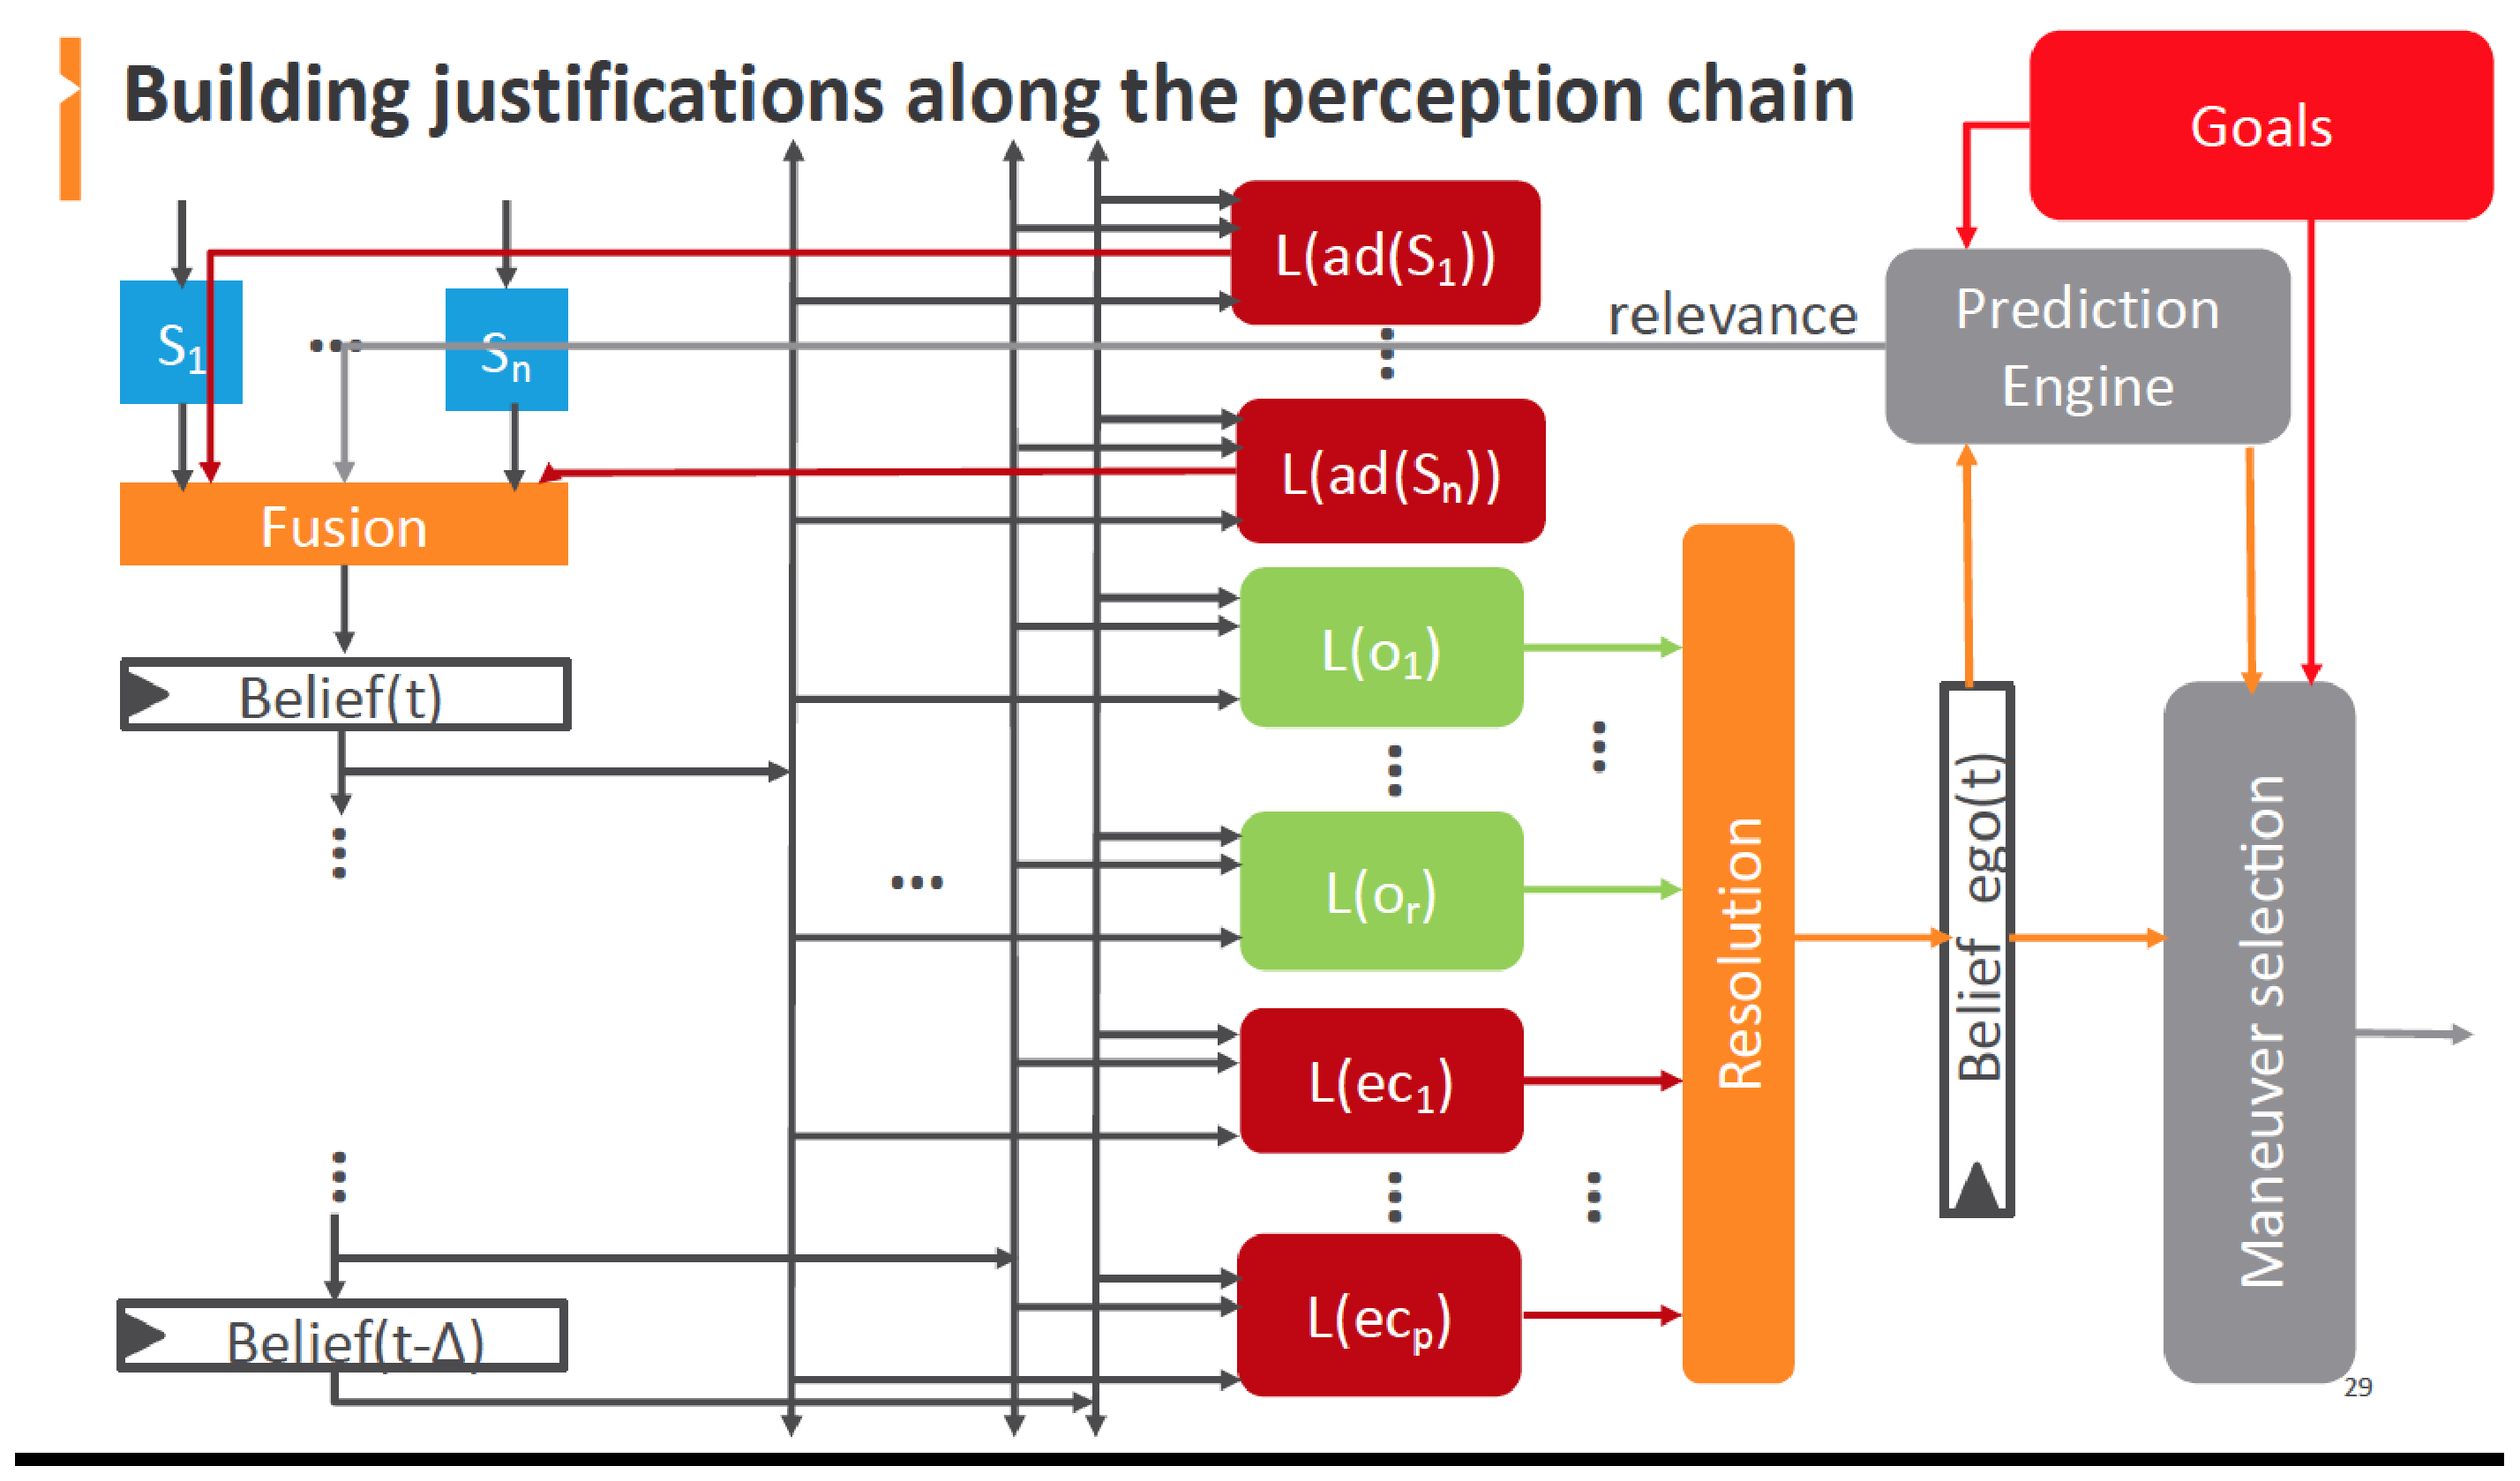
\includegraphics[width=\textwidth]{fig2.eps}
    \caption{Reference architecture}
    \label{fig:architecture}
\end{figure}
Figure \ref{fig:architecture} shows the proposed functional reference architecture of the perception chain, where \textit{belief(t)} represents the labelled occupancy grid resulting from fusion of sensors s1 to sn, as discussed previously. We distinguish these from the complete reconstruction of the environment of the ego car, \textit{belief(ego)}, and assume that for each artifact  $a$ in the ontology we have a dedicated learning component  $L(a)$ for detecting \emph{both presence and absence of $a$} in fields of the occupancy grid, see below. A prediction engine provides feedback about the relevance of fields in the occupancy grid, based on knowledge about the current beliefs of the ego car, and its current goals, as elaborated below. Note that the learning components for identifying adverse sensor conditions are fed backwards into the sensor fusion unit. We propose the following measures to reduce the error of misperception:
\begin{enumerate}
\item To be able to exploit physical laws to optimize the prediction rate, we propose to maintain copies of such beliefs over some time window $\Delta$, and feed this into the classification network. Thus e.g. in the resolution phase we can flag an incorrect classification of pedestrians, if the artifacts misclassified as pedestrians cross a four-lane street in one second.
\item We require for each learning component $L(a)$ and each occupied field of the occupancy grid as determined by sensor fusion to output both \emph{strength of beliefs for presence and for absence of $a$}. We will only pass on classification votes of $L(a)$ into beliefs of ego in the resolution process, if such strength values are separated by a safety margin determined by the criticality of misclassification for either ensuring presence of $a$ or absence of $a$ in a given field of the occupancy grid, as determined by the prediction engine. Such safety margins are thus adapted dynamically, by optimizing threshold values so as to maximize availability as long as criticality dependent errors of misclassification are achieved.
\item We use the ordering relation of the ontology to detect misclassifications in the resolution phase. E.g. identifying simultaneously a car and a pedestrian at the same location is impossible, unless both a car and a pedestrian were within reach to this location in the previous belief, taking into account the laws of physics captured in the respective behavioral models. Similarly, we detect inconsistencies in classification for ordered elements in the ontology, e.g. identifying a racing car while at the same time claiming that the same location does not contain a car.
\item We propose in-the-field learning for adverse conditions, by constantly comparing the individual sensors perception of the occupancy grid with the result from sensor fusion, including detection of inconsistencies. Under current regulation, such an on-line learning process must be done on a separate copy of the network, subject to off-line verification and validation prior to activation.
\end{enumerate}

As a result of the resolution process, the current beliefs of ego contain a complete characterization of the electronic horizon in terms of observables defined by the ontology, where each non-bottom perception is decorated with the maximal risk of misperception.

We assume that the ego vehicle is pursuing a finite, possibly dynamically changing, set of goals, e.g. expressed as linear temporal logic (LTL) formulas over the observables of $TS(ego)$. The importance of achieving a given goal $g$ is expressed by a cost function $C(g)$. For safety requirements, we assume that these are split according to ISO 26262 severity categories, with costs determined e.g. based on costs determined by HSE for the corresponding MAIS categories, thus costs reflect the incurred penalty of not achieving this goals. Safety related goals are always active, as are (lower priority) goals requiring availability. Such static goals are enriched by situation dependent goals, also decorated with costs.

The prediction component takes into account
\modify{\begin{itemize}
\item the current belief of the ego vehicle
\item the current weather conditions
\item the current road configuration and road condition
\item the current best classification $a$ of all relevant traffic participants
\item  the dynamic model characterizing the behaviour of such traffic participants in such operational contexts, as given by $cl(a)$
\item the current set of goals
\end{itemize}}{ the current belief of the ego vehicle, the current weather conditions, the current road configuration and road condition, the current best classification $a$ of all relevant traffic participants, the dynamic model characterizing the behaviour of such traffic participants in such operational contexts, as given by $cl(a)$, the current set of goals,
}
and determines on this basis at each time instance $t_j$ a set of candidate manoeuvres $cm(t_j)$  minimizing the penalty resulting from the sum of penalties of goals not achievable by a given set of maneuvers. For each $m\in cm(t_j)$, let $G(m)$ be the subset of goals considered achievable by the prediction component, if maneuver $m$ can be executed successfully. The design of such a prediction component is a core competence of the OEM and not restricted by the reference architecture. Instead, the reference architecture provides for a feedback-loop to the perception chain: for each maneuver $m\in cm(t_j)$, the perception component can determine with which precision the perception engine must answer queries at time $t_{j+1}$. Such queries take the form of a Boolean expression over both labels and classification on subspaces of the occupancy grid, testing both preconditions and invariants of the maneuver required for its successful completion. We denote by $ba(m)$ the query enabling maneuver $m$. It is decorated by a maximally tolerated rate of misprediction $p_m$, which is canonically derived from the costs of failing to achieve $G(m)$. Hence at time $t_{j+1}$, the set of all such decorated queries characterizes the relevant subspaces, labels, and classifications of the occupancy grid. 

